\documentclass{report}
\usepackage{sbc-template}
\usepackage{graphicx}
\usepackage[utf8]{inputenc}
\usepackage[T1]{fontenc}
\usepackage{pgfplots}
\usepackage{pgfplotstable} 
\usepackage{titlesec}
\usepackage{lipsum}
\usepackage{authblk}
\usepackage{mathtools}
\DeclarePairedDelimiter{\ceil}{\lceil}{\rceil}
\renewcommand{\contentsname}{Sumário}

\titleformat{\chapter}[display]{\normalfont\bfseries}{}{0pt}{\Large}

\begin{document}

\title{Recuperação de Informação - Máquinas de Busca na Web: Trabalho Prático 2}
\author{João Mateus de Freitas Veneroso}
\affil{Departamento de Ciência da Computação da Universidade Federal de Minas Gerais}

\maketitle

\tableofcontents

\chapter{Introdução}

O índice invertido é uma estrutura de dados que mapeia termos aos locais onde eles ocorrem
dentro de uma coleção de documentos. Esta estratégia de indexação exige um pré-processamento
significativo da coleção, no entanto, ela é muito eficiente para retornar resultados precisos
em tempo de busca. Este relatório descreve a implementação de um índice invertido em C++ e
os experimentos realizados com base em uma coleção com aproximadamente 650 GB de documentos
primariamente em português coletados na web. A versão mais recente do código pode ser obtida
em: https://github.com/jmfveneroso/inverted-index. Para instruções de compilação e uso, leia
o arquivo README.md. 

\chapter{Índice invertido}
O objetivo deste projeto era implementar uma ferramenta eficiente de construção de índices 
invertidos (inversor) por meio da utilização de ordenação externa. O inversor construído
utilizou ordenação externa com um bloco de memória principal de 600 MB, intercalação
inplace e compressão das listas de apontadores por meio do método $ Elias-\delta $. O processo
de funcionamento da ferramente de inversão pode ser descrito em quatro etapas:

\begin{description}
  \item [Extração]    O inversor percorre a coleção e armazena os termos encontrados e suas posições em triplas.
  \item [Ordenação]   As triplas coletadas na etapa de extração são ordenadas por meio do algoritmo de ordenação externa.
  \item [Compressão]  As triplas ordenadas são comprimidas por meio da utilização do método $ Elias-\delta $.
  \item [Finalização] As estruturas auxiliares são escritas no arquivo invertido.
\end{description}

\section{Extração}

Durante a etapa de extração, o inversor percorre toda a coleção de documentos e, para cada documento, guarda
a posição do documento na coleção (id do documento), o arquivo em que o documento se encontra e o offset
em relação ao começo do arquivo. Isso permite que, em tempo de busca, seja possível encontrar o conteúdo exato
dos documentos da coleção com base nos termos que neles ocorrem. Além disso, para cada termo de 
cada documento, o inversor salva triplas com o seguinte formato no arquivo invertido: \newline

\[ < \textit{id do termo}; \textit{id do documento}; \textit{posição do termo} > \]

Cada novo termo encontrado é armazenado no Lexicon e uma id única é atribuída à ele. O inversor
normaliza os termos retirando acentos e convertendo todos os caracteres para sua versão minúscula. Além disso,
caracteres não alfa numéricos são considerados separadores, portanto, não são indexados. Cabe ressaltar que
documentos provindos da web podem possuir padrões de codificação diversos, o que dificulta o tratamento universal
de caracteres especiais. A etapa de tratamento destes padrões de codificação foi delegada à biblioteca externa
gumbo-parser (https://github.com/google/gumbo-parser) e, dessa forma, todos os caracteres da coleção foram
tratados no formato UTF-8. A biblioteca gumbo-parser é bastante resiliente em relação à HTML defeituoso, no entanto,
ela não funciona bem como parser universal de XML, portanto, os documentos XML presentes na coleção foram ignorados. 
Isso não representou grande perda, pois, a maior parte destes documentos eram feeds RSS. A
biblioteca htmlcxx sugerida é cerca de duas vezes mais rápida que o gumbo-parser, no entanto, ela não lida bem com os
diferentes padrões de codificação, tem documentação ruim e não é mantida pela comunidade, por isso, o gumbo-parser
foi a escolha final.

O extrator acumula as triplas em um bloco de memória principal até que o bloco fique cheio e, então, o bloco inteiro
é ordenado e então é escrito no arquivo invertido. Desta forma, ao final da etapa de extração, o arquivo invertido
contém k blocos de triplas ordenadas. Onde:

\[ k = \ceil[\Big]{\frac{\textit{triplas na coleção}}{\textit{triplas por bloco}}} \]

Sendo que o número de triplas por bloco depende da quantidade de memória principal utilizada.
Se o último bloco da coleção não estiver cheio ao final do último documento, o restante do bloco é preenchido com 
um padding de triplas nulas <0, 0, 0>. As ids de termos, ids de documentos e posições de palavras são sempre maiores que 0, 
portanto, estas triplas são inválidas.

A coleção indexada neste trabalho apresentava alguns problemas. Documentos com URLs duplicadas no seguinte formato: 
"http://exemplo/" e "http://exemplo//" apareceram com certa frequência, nesse caso, a segunda ocorrência do documento foi ignorada.
O mesmo tratamento foi dado para URLs cujo formato canônico era idêntico. Além disso, em alguns arquivos havia URLs
com pipes "|", por exemplo: "http://exemplo/id=|x|/". Nesse caso, a primeira ocorrência do pipe foi considerada o separador
e as próximas ocorrências antes do pipe triplo que sinaliza o final do documento foram consideradas conteúdo. Por último,
alguns documentos utilizavam um padrão de codificação desconhecido e, neste caso, os caracteres acentuados ficaram prejudicados.

\begin{table}
\centering
\begin{tabular}{ |l|l| }
  \hline
  \multicolumn{2}{|c|}{Etapa de extração} \\
  \hline
  Número de triplas extraídas & 9.340.391.824 \\
  Tamanho da tripla & 12 bytes \\
  Tamanho do bloco em memória principal & 600 MB \\
  Triplas por bloco & 50 milhões \\
  Número total de blocos & 187 \\
  Padding do último bloco (triplas) & 9.608.176 \\
  Número de termos na coleção & 18.498.889 \\
  Número de documentos válidos & 8.110.563 \\
  Triplas por documento & 1151.63 \\
  Tempo total & 14,26 horas \\
  Velocidade de extração por documento (ms) & 6.33 ms \\
  Tamanho do arquivo gerado & 112,08 GB \\
  \hline
\end{tabular}
\caption{Extração}
\label{tab:extractor}
\end{table}

Os dados da coleção de triplas obtida ao final da etapa de extração podem ser conferidos na tabela \ref{tab:extractor}. De acordo
com o profiling realizado, mais de 90\% do tempo de execução foi gasto na etapa de parsing dos documentos, portanto, melhorias
no código teriam de considerar uma outra estratégia de parsing. A complexidade assintótica da etapa de ordenação é O(n) para o 
parsing, com n referente ao número de bytes na coleção. A complexidade da ordenação dos blocos é $ O(\frac{n}{k}log(\frac{n}{k})) $
por bloco e  $ O(nlog(\frac{n}{k})) $ no total, onde k é o número de blocos e n o número de triplas extraídas. A complexidade de espaço 
em memória secundária é O(n) para as triplas extraídas. E a complexidade de espaço em memória principal é $ O(\frac{n}{k}) $, 
referente ao tamanho do bloco de triplas.

\section{Ordenação}

Em posse dos blocos ordenados produzidos na etapa de extração, resta ordenar as triplas universalmente.
Para tanto, foi utilizada uma estratégia de ordenação externa. Além disso, foi feita a intercalação inplace
de forma a salvar um pouco de espaço em disco.

\subsection{Ordenação externa}

A intercalação das tuplas da coleção completa utilizou 600 MB de memória principal, equivalente à 50 milhões de triplas. 
Inicialmente, cada um dos 187 blocos teve uma parte igual de suas triplas (267.379) transferido para memória principal, o que soma um total de
49.999.873 triplas. A partir daí, as triplas foram inseridas em uma heap e então retiradas uma a uma e escritas em sua posição final (considerando
que ainda será feita a intercalação inplace). Sempre que o número de triplas em memória principal de um determinado bloco se exauria, uma nova leva
de 267.379 triplas era extraída daquele bloco até que o bloco se tornasse vazio. Quando o bloco
se tornava vazio, ele poderia ser preenchido com triplas em sua ordenação final de acordo com os critérios da intercalação inplace, que será descrita logo
adiante. A ordenação extrena é mais eficiente quanto maior for o tamanho do bloco de memória principal utilizado.

A complexidade da ordenação externa é $ O(nlog n) $, onde n é o número de triplas extraídas da coleção, e utilizando uma heap
binária, cuja com complexidade de pior caso para a inserção e remoção é igual a $ O(log n)$.

\subsection{Intercalação inplace}

A diferença básica entre a intercalação normal e a intercalação inplace é que a intercalação inplace utiliza os
espaços deixados pelos blocos vazios para escrever as triplas em sua ordenação final e, quando não existem blocos vazios,
um bloco extra é criado ao final de todos os blocos. No caso deste trabalho, as triplas ordenadadas universalmente são divididas em 187
segmentos que devem ser colocados em suas posições finais após a ordenação. Assim, a medida que a ordenação externa acontece, 
cada vez que um destes segmentos é gerado, ele é escrito em um bloco vazio ou bloco extra e a relação entre a posição verdadeira 
deste segmento e sua posição atual é mantida em um mapa.
Ao final, o mapa é percorrido reordenando estes segmentos e, durante esta etapa, é feita a compressão das listas de apontadores, que será
melhor descrita na próxima sessão.

É interessante notar que, quanto melhor distribuídos estiverem os termos entre os documentos, ou seja, quanto maior for a entropia, 
menos eficiente será a intercalação inplace. Pois, vários blocos demorarão a ficar vazios e será necessário criar mais blocos extras.

A complexidade da intercalação inplace é $ O(k) $, onde k é o número de blocos.

\begin{table}
\centering
\begin{tabular}{ |l|l| }
  \hline
  \multicolumn{2}{|c|}{Etapa de ordenação} \\
  \hline
  Número de triplas em memória principal & 50 milhões \\
  Tamanho do bloco em memória principal & 600 MB \\
  Triplas por bloco em memória principal & 267.379 \\
  Número de blocos & 187 \\
  Número de blocos extras & 180 \\
  Tempo total & 10.52 horas \\
  \hline
\end{tabular}
\caption{Ordenação}
\label{tab:sort}
\end{table}

Os dados da etapa de ordenação estão descritos na tabela \ref{tab:sort}.

\section{Compressão}

As listas de apontadores finais do arquivo invertido foram comprimidas com base nos intervalos entre ids de documentos e posição
das palavras nas triplas de um determinado termo. Portanto, para cada termo, as listas tinham o seguinte formato:

\[ < dgap_i; freq_i; tgap_{i1}, tgap_{i2}, ..., dgap_j, freq_j, tgap_{j1}, tgap_{j2}, ... >\]

Onde, $ dgap_i $ representa o intervalo entre a id do documento i e o documento anterior na lista de apontadores (no caso do primeiro documento
é a distância em relação à zero), $ freq_i $ representa a frequência do termo no documento i e $ tgap_{ik} $ representa a posição k em que o termo 
ocorre no documento i.

\begin{table}
\centering
\begin{tabular}{ |l|l| }
  \hline
  \multicolumn{2}{|c|}{Etapa de compressão} \\
  \hline
  Espaço ocupado pelas triplas antes da compressão & 112,08 GB \\
  Espaço ocupado após a compressão & 18 GB \\
  Razão de compressão & 16,05\% \\
  Tempo total para intercalação inplace e compressão & 5,24 horas \\
  \hline
\end{tabular}
\caption{Compressão}
\label{tab:compression}
\end{table}

Para cada uma das listas de apontadores no formato descrito, os valores dos $ dgaps $ e $ tgaps $ são comprimidos com base no algoritmo $ Elias-\delta $.
É importante lembrar que os offsets das listas de cada termo e as frequências dos termos na coleção são armazenados para serem salvos na etapa de finalização.
Como a compressão é feita durante a intercalação inplace, o tempo total da compressão é somado à intercalação inplace. Os dados da etapa de compressão
estão descritos na tabela \ref{tab:compression}. A razão de compressão final ficou em 16.05\%, no entanto, é necessário lembrar que cada tripla contém 
a id do termo, que poderia ser removida nas listas de apontadores, uma vez que dentro de uma lista, todos os apontadores se referem ao mesmo termo. Portanto, 
um terço da compressão se dá por esse fato. O restante é o ganho real do algoritmo $ Elias-\delta $.

A complexidade da compressão é $ O(n) $, onde n é o número de triplas extraídas da coleção.

\section{Finalização}

\begin{table}
\centering
\begin{tabular}{ |l|l| }
  \hline
  \multicolumn{2}{|c|}{Estrutura do arquivo invertido} \\
  \hline
  Seção & Espaço \\
  \hline
  Header & 24 bytes \\
  Listas de apontadores & 18 GB \\
  Mapa de documentos & 728 MB \\
  Lexicon & 772 MB \\
  \hline
\end{tabular}
\caption{Arquivo invertido}
\label{tab:inverted_file}
\end{table}

A etapa de finalização escreve as estruturas auxiliares no arquivo invertido: o header, o lexicon e o mapa de documentos.
O lexicon contém todos os termos encontrados, além de informações como os offsets para as listas de apontadores no arquivo invertido
e a frequência dos termos na coleção. O lexicon da coleção inteira ocupou 772 MB.
O mapa de documentos guarda para cada documento: a URL, o arquivo do qual o documento foi extraído e o offset para o início do documento. 
O mapa de documentos da coleção inteira ocupou 728 MB.
O header contém informações sobre o número de termos encontrados, o número de documentos, e os offsets para o começo do lexicon e do mapa de documentos.

Ao fim do processo de inversão, o arquivo invertido reproduz a estrutura descrita na tabela \ref{tab:inverted_file}.
Além das informações aqui descritas, o arquivo invertido também conta com o índice de anchor texts, as normas dos vetores dos documentos e seu page rank. 
No entanto, o processo de escrita destas estruturas não será descrito neste relatório pois não é objeto deste trabalho prático.

A complexidade da etapa de finalização é $ O(n + m) $, onde n é o número de termos na coleção e m o número de documentos. Somando-se todas as etapas,
a complexidade da criação do índice invertido é $ O(nlog n) $, onde n é o número de triplas extraídas, pois, em todos os casos, as outras quantidades 
variáveis da coleção são muito menores do que o número de triplas.

\chapter{Experimentos}

Os experimentos deste projeto consistiram em: criar o arquivo invertido de uma coleção de cerca de ~650 GB de documentos da web, realizar buscas no índice 
construído e testar o tempo gasto na etapa de ordenação das triplas dada a quantidade de memória principal utilizada. Todos os experimento foram realizado 
em um computador com disco rídigo SATA Rev 3.0 de 1 TB, processador Intel(R) Core(TM) i5-4460 3.20GHz e 16 GB RAM.

\section{Inversão da coleção completa}

\begin{figure}
\centering
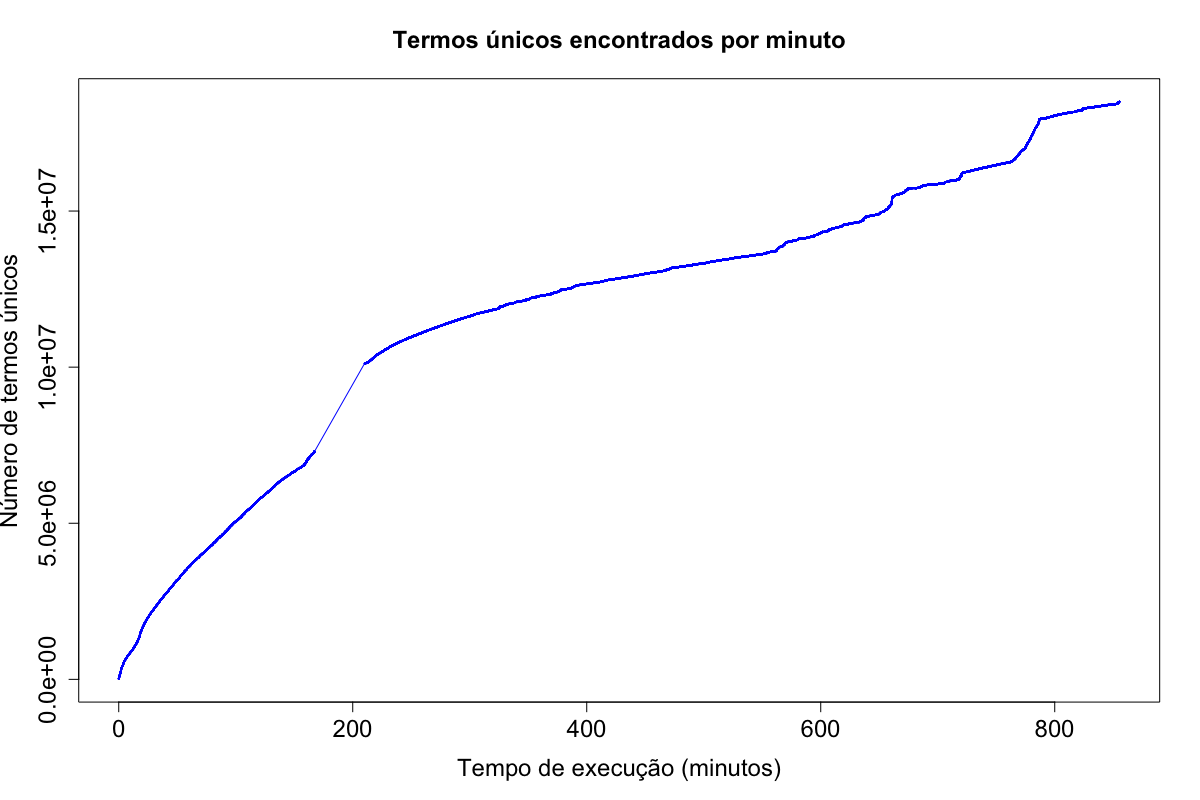
\includegraphics[width=\linewidth]{lexemes.png}
\label{fig:lexemes}
\caption{Termos únicos encontrados por minuto na etapa de extração} 
\end{figure}

\begin{figure}
\centering
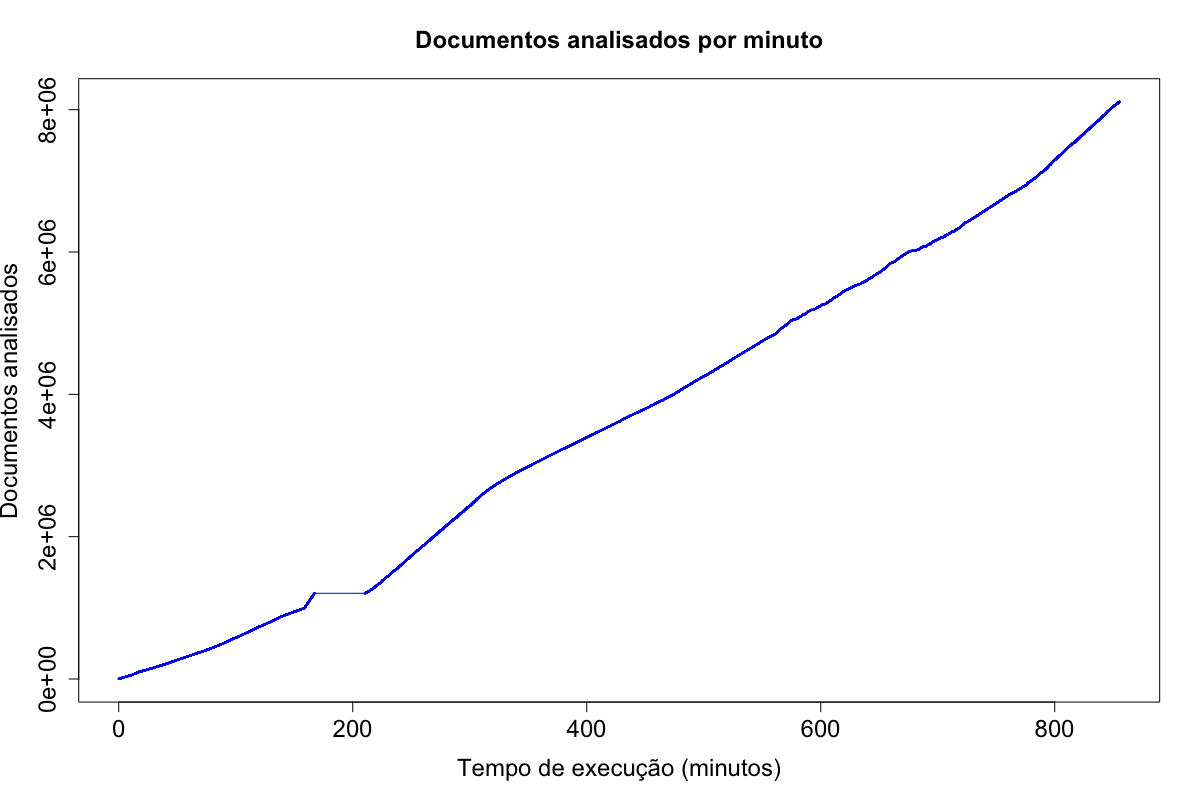
\includegraphics[width=\linewidth]{extractor.png}
\label{fig:extractor}
\caption{Documentos analisados por minuto na etapa de extração} 
\end{figure}

A construção do índice invertido para a coleção completa durou ao todo cerca de 30 horas, sendo que a etapa de extração durou 14,26 horas, a etapa de ordenação durou 10,52 horas e a compressão das listas de apontadores durou 5,24 horas. O gráfico \ref{fig:lexemes} mostra a quantidade de termos únicos encontrados por minuto na etapa de extração. Percebe-se que o ritmo de descoberta de termos novos diminui a medida que se avança na coleção. Isso acontece porque os termos mais utilizados são descobertos cedo e, a medida
que cresce o numero de termos no lexicon, se torna mais difícil encontrar termos novos. O gráfico 3.2 mostra o número de documentos analisados
por minuto na etapa de extração. Houve um problema com a coleta dos dados próximo ao minuto 200 e como o experimento é muito longo não foi possível repetí-lo. 
No entanto, as conclusões gerais não ficam muito prejudicadas por esta perda de informação.

\section{Buscas}

\begin{table}
\centering
\begin{tabular}{ |l|l|l|l| }
  \hline
  \multicolumn{4}{|c|}{Buscas no arquivo invertido} \\
  \hline
  Termo          & Tempo (ms)     & Número de documentos & Frequência Total \\
  \hline                             
  recuperação    & 11925          & 62.614               & 114.825          \\
  máquinas       & 27889          & 96.643               & 206.463          \\
  web            & 1840095        & 811.475              & 1.944.708        \\               
  ciência        & 61501          & 144.861              & 337.712          \\               
  computação     & 2767           & 28.530               & 64.348           \\              
  ufmg           & 3802           & 34.024               & 139.880          \\               
  gumbo          & 46             & 1.349                & 2.095            \\               
  github         & 763            & 13.780               & 26.483           \\               
  java           & 9657           & 55.588               & 190.031          \\               
  python         & 1448           & 19.679               & 69.241           \\               
  \hline
\end{tabular}
\caption{Buscas}
\label{tab:search}
\end{table}

Antes de iniciar o buscador, é necessário carregar em memória as estruturas auxiliares do índice invertido: o lexicon e o mapa de documentos. Este processo
leva aproximadamente 220 segundos.

Para conferir a qualidade do índice gerado no primeiro experimento, foram realizadas 10 buscas cujos resultados estão descritos
na tabela \ref{tab:search}, a tabela descreve o tempo para listar todos os documentos onde o termo aparece, o número de documentos onde o termo
aparece e a frequência total do termo na coleção. Um exemplo de saída do buscador foi salvo na root do projeto com o nome search.log.

\section{Ordenação X Memória principal}

\begin{table}
\centering
\begin{tabular}{ |l|l|l| }
  \hline
  \multicolumn{3}{|c|}{Velocidade de ordenação} \\
  \hline
  Tamanho do bloco & Número de blocos & Tempo (ms) \\
  \hline                             
  10 MB            & 65               & 233106 \\
  20 MB            & 33               & 220774 \\
  30 MB            & 22               & 220127 \\               
  40 MB            & 15               & 278959 \\               
  50 MB            & 13               & 211959 \\              
  100 MB           & 7                & 223152 \\               
  200 MB           & 4                & 247336 \\               
  300 MB           & 2                & 285716 \\               
  400 MB           & 2                & 235183 \\
  500 MB           & 2                & 302967 \\               
  \hline
\end{tabular}
\caption{Velocidade X Memória Principal}
\label{tab:sorter}
\end{table}

A tabela \ref{tab:sorter} mostra a velocidade de ordenação das triplas conforme o tamanho do bloco de memória principal utilizado. O experimento foi
realizado com uma parte reduzida da coleção completa contendo 50.018 documentos, 852.285 termos e 53.630.256 triplas. O tamanho do bloco de memória
principal utilizado variou entre 10MB e 500MB. É possível perceber uma pequena melhora com o crescimento do tamanho do bloco até ~100 MB, a piora
posterior provavelmente acontece por conta do crescimento do padding. O resultado deste teste não foi muito revelador. A melhora na velocidade de 
ordenação provavelmente seria mais acentuada caso a coleção de teste fosse maior. Como a coleção é pequena, os custos fixos e instabilidades na 
velocidade de processamento acabam prejudicando o resultado observado.

\chapter{Conclusão}

O objetivo deste trabalho era construir um índice invertido para a combinação das coleções obtidas no
Trabalho Prático 1 e esse índice foi construído com sucesso em um tempo total de 30 horas. O índice da coleção final
tem o tamanho de 16 GB (comprimido no formato tar.gz) e pode ser conferido em: \newline
visconde.latin.dcc.ufmg.br:/mnt/hd0/joao\_test/inverted\_index.data.tar.gz.

\end{document}
